\documentclass[a4paper,12pt]{article}
\usepackage{amsmath}
\usepackage{graphicx}
\usepackage{listings}
\usepackage{caption}
\usepackage{hyperref}
\usepackage{booktabs}
\usepackage{pgfplots} % For including plots
\usepackage{ragged2e}
\usepackage{listings}
\usepackage{float}
\usepackage{geometry}
\usepackage{wrapfig} % Required for wrapping text around figures
\geometry{margin=2.5cm} % <-- Set all margins to 2.5cm. Change as needed.
\usepackage[most]{tcolorbox}

\usepackage{graphicx} % For including images
\usepackage{caption}    % For customized captions
\usepackage{subcaption} % For subfigures (multiple images in one figure environment)
\usepackage{float}      % For more control over float placement, e.g., [H]
% Adjust geometry if needed for better page layout with many images
% \usepackage[margin=2.5cm]{geometry}


\hypersetup{
    hidelinks
}


\usepackage{xcolor}

\definecolor{codegreen}{rgb}{0,0.6,0}
\definecolor{codegray}{rgb}{0.5,0.5,0.5}
\definecolor{codepurple}{rgb}{0.58,0,0.82}
\definecolor{backcolour}{rgb}{0.95,0.95,0.92}

\tcbset{
    frame code={},
    center title,
    left=0pt,
    right=0pt,
    top=0pt,
    bottom=0pt,
    colback=backcolour,
    colframe=white,
    width=\dimexpr\textwidth\relax,
    enlarge left by=0mm,
    boxsep=5pt,
    arc=0pt,outer arc=0pt,
    }



\lstdefinestyle{mystyle}{
    backgroundcolor=\color{backcolour},   
    commentstyle=\color{codegreen},
    keywordstyle=\color{magenta},
    numberstyle=\tiny\color{codegray},
    stringstyle=\color{codepurple},
    basicstyle=\ttfamily\footnotesize,
    breakatwhitespace=false,         
    breaklines=true,                 
    captionpos=b,                    
    keepspaces=true,                 
    numbers=left,                    
    numbersep=5pt,                  
    showspaces=false,                
    showstringspaces=false,
    showtabs=false,                  
    tabsize=2
}

\lstset{style=mystyle}

\usepackage{graphicx} % Required for inserting images

\title{Artificial Intelligence and Machine Learning}
\author{Cliffwalking}
\date{Authors:\\Alessandro Rocchi\\Onorio Iacobelli}

\begin{document}

\maketitle

\tableofcontents

\section{Introduction}
In this Machine Learning project we will focus on the subject of Reinforcement Learning applied to the "Cliff Walking" environment. The goal of the agent is to reach a specified location, by moving in the four directions without falling down the cliff. This problem represents a fundamental challenge in Reinforcement Learning, combining elements of exploration/exploitation tradeoff, temporal credit assignment and policy optimization. This environment provides an excellent testbed for comparing different Reinforcement Learning approaches, in particular tabular Q-learning and Deep Q-Networks (DQN).
\vspace{0,5cm}\\
Our implementation explores both classical tabular methods, suitable for discrete state spaces and modern deep learning approaches that can handle more complex scenarios. Trough extensive experimentation and hyperparameter tuning, we demonstrate how different choices and configurations impact learning performance and convergence behavior. 
\section{Reinforcement Learning}
Reinforcement Learning is a branch of machine learning focused on decision making trough interaction with the environment. Unlike supervised learning, where the correct outputs are given for training, in Reinforcement Learning the agent must discover the optimal behavior by trial and error, guided only by rewards. Formally, Reinforcement Learning is often modeled as a Markov Decision Process (MDP), defined by states, actions, transition probabilities and rewards. The agent's goal is to learn a policy, a mapping from states to actions, that maximizes the expected cumulative reward over time.
\vspace{0,5cm}\\
The core components of a Markov Decision Process are:
\begin{itemize}
    \item \textbf{Agent}: the learner or decision-maker that interacts with the environment. In our case this is the entity navigating the cliff walking grid.
    \item \textbf{Environment}: the external system that the agent interacts with. For cliff walking, this includes the grid world, cliff locations, and reward structure.
    \item \textbf{State (S)}: a representation of the current situation in the environment. In cliff walking, this is the agent's current position in the grid.
    \item \textbf{Action (A)}: the choices available to the agent at any given state.
    \item \textbf{Reward (R)}: the feedback signal from the environment indicating how good or bad the last action was. Rewards guide the learning process.
    \item \textbf{Policy ($\pi$)}: the agent's strategy for choosing actions given states. This can be deterministic (always choose the same action in a given state) or stochastic (choose actions according to a probability distribution).
    \item $\delta(s'|s,a)$: the probability distribution over the transitions.
\end{itemize}
The Reinforcement Learning process follows a continuous loop:
\begin{enumerate}
    \item Observe the current state of the environment
    \item Select an action based on the current policy
    \item Execute the action in the environment
    \item Receive a reward and observe the new state
    \item Update the policy based on the experience
    \item Repeat until learning converges or a stopping criterion is met
\end{enumerate}
One of the fundamental challenges in Reinforcement Learning is balancing \textbf{exploration} (trying new actions to discover potentially better strategies) with \textbf{exploitation} (using known good actions to maximize rewards). This balancing is crucial because too much exploration can lead to the agent wasting time on suboptimal actions, on the other hand with too little exploration the agent may get stuck in a local optimum and never discover the best strategy.
\subsection{Q-Learning}
Q-Learning is a model-free Reinforcement Learning algorithm that learns the quality of actions, telling the agent what actions to take under what circumstances. The "Q" stands for quality, representing the expected future reward for taking a specific action in a specific state.\\ The \textbf{Q-function} Q(s,a) represents the expected cumulative reward when taking action 'a' in state 's' and then following the optimal policy. The learning process involves iteratively updating these Q-values using the Bellman equation:
\begin{figure}[H]
    \centering
    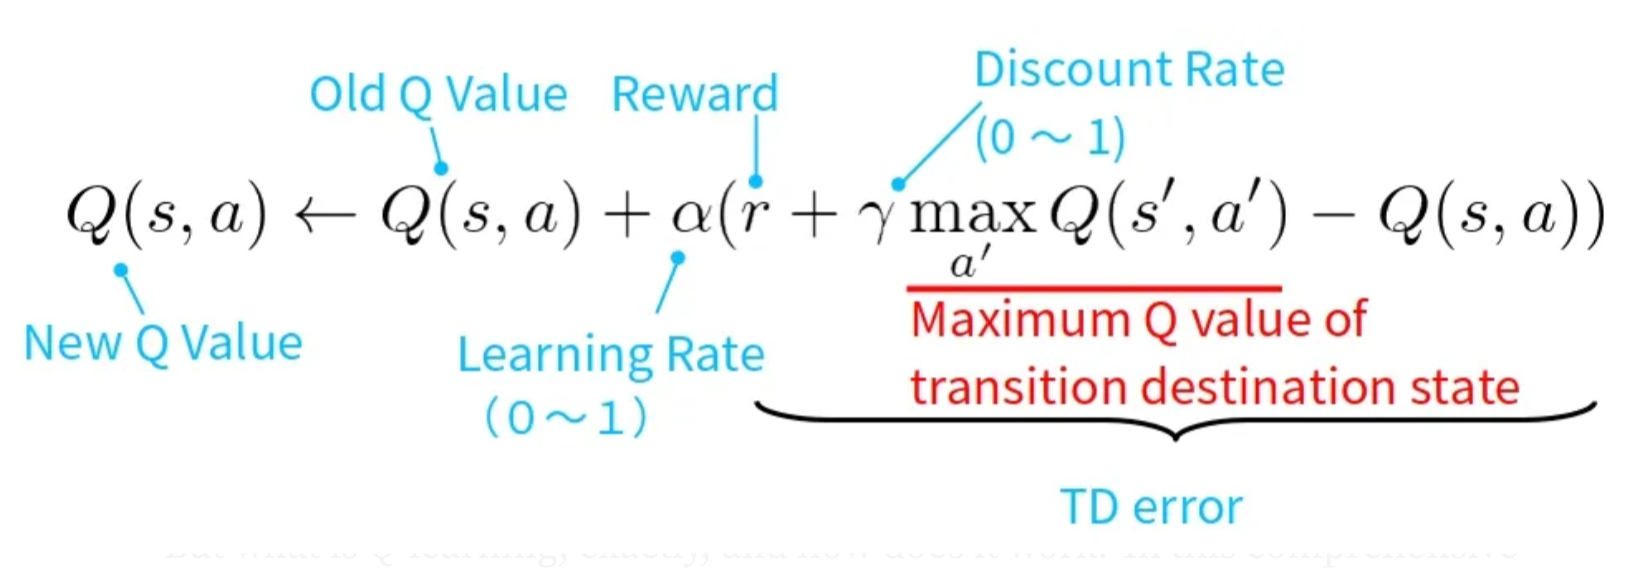
\includegraphics[scale=0.5]{bellman.png}
\end{figure}
Where:
\begin{itemize}
    \item \textbf{$\alpha$ (alpha)}: learning rate controlling how quickly new information overrides old information
    \item \textbf{r}: immediate reward received
    \item \textbf{$\gamma$ (gamma)}: discount factor determining the importance of future rewards
    \item \textbf{s'}: next state after taking action 'a' in state 's'
\end{itemize}
\textbf{Tabular Q-Learning} maintains explicit Q-values for every (state, actions) pair in a lookup table. This approach works well for environments with small, discrete state and action spaces but becomes impractical as the state space grows.
\vspace{0,5cm}\\
\textbf{Deep Q-Networks (DQN)} use neural networks to approximate the Q-function, enabling the handling of large or continuous state spaces. Instead of storing individual Q-values, the network learns to map states to Q-values for all possible actions.
\vspace{0,5cm}\\
To balance exploration and exploitation, we implement an epsilon-greedy policy:
\begin{itemize}
    \item With probability \textbf{$\varepsilon$ (epsilon)}: choose a random action (exploration)
    \item With probability \textbf{(1-$\varepsilon$)}: choose the action with the highest Q-value (exploitation)
\end{itemize}
The epsilon value starts high (encouraging exploration) and gradually decreases (shifting toward exploitation) as learning progresses.
\section{Environment}
The Cliff Walking environment is part of the Toy Text environments which contains general information about the environment. It involves crossing a grid world from start to goal while avoiding falling off a cliff.
\begin{figure}[H]
    \centering
    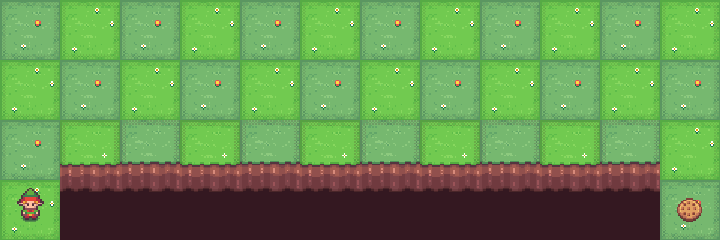
\includegraphics[scale=0.7]{cliff_walking.png}
\end{figure}
\subsection{Description}
The game starts with the player at location [3, 0] of the 4x12 grid world with the goal located at [3, 11]. If the player reaches the goal the episode ends.
\vspace{0,5cm}\\
A cliff runs along [3, 1..10]. If the player moves to a cliff location it returns to the start location.
\vspace{0,5cm}\\
The player makes moves until they reach the goal.
\subsection{Action Space}
The action shape is (1,) in the range \{0, 3\} indicating which direction to move the player.
\begin{itemize}
    \item 0: Move up
    \item 1: Move right
    \item 2: Move down
    \item 3: Move left
\end{itemize}
Actions that would move the agent outside the grid boundaries result in no movement (the agent stays in the same position).
\subsection{Observation Space}
There are 3 x 12 + 1 possible states. The player cannot be at the cliff, nor at the goal as the latter results in the end of the episode. What remains are all the positions of the first 3 rows plus the bottom-left cell.
\vspace{0,5cm}\\
The observation is a value representing the player’s current position as current\_row * ncols + current\_col (where both the row and col start at 0).\\For example, the starting position can be calculated as follows: 3 * 12 + 0 = 36.
\vspace{0,5cm}\\
The observation is returned as an int().
\subsection{Reward}
The reward system is designed to encourage finding the shortest safe path while severely penalizing dangerous moves:
\begin{itemize}
    \item \textbf{Standard step}: -1 reward (encourages shorter paths)
    \item \textbf{Falling off cliff}: -100 reward + episode termination
    \item \textbf{Reaching goal}: 0 reward + episode termination
\end{itemize}
This reward structure creates an interesting dilemma: the shortest path (along the cliff edge) is risky but potentially more rewarding if executed perfectly, while the safe path (around the cliff) is longer but more reliable.
\vspace{0,5cm}\\
The episode terminates when the Agent reaches the goal position, falls of the cliff or the episode can exceeds maximum step limit.
\section{Models Adopted}

\end{document}